
\documentclass{../templates/llncs}
\usepackage{../templates/salt-light}
\usepackage{makeidx}
\usepackage{url}
\usepackage{graphicx}
\usepackage{array}

\begin{document}

\title{Cooking HTTP content negotiation with Vapour} % FIXME

\author{Diego Berrueta\inst{1}, Sergio Fern\'andez\inst{1} and Iv\'an Frade\inst{2}}

\institute{
Fundaci\'on CTIC\\
Gij\'on, Asturias, Spain\\
\email{\{diego.berrueta,sergio.fernandez\}@fundacionctic.org\\http://www.fundacionctic.org/}
\and
Universidad de Oviedo\\
Oviedo, Asturias, Spain\\
\email{ivan.frade@gmail.com\\http://www.uniovi.es/}
}

\maketitle

\begin{abstract}
The Semantic Web is built upon distributed knowledge published on 
the Web. But this vision can not be implemented without some basic publishing
rules to make machine-understandable this data. Special mention must be 
given to the publication of RDF vocabularies for the importance that they have 
in the Semantic Web architecture. In this paper we describe a scripting 
web-based application that validates the compliance of a published vocabulary 
against these rules. We think that practical experimentation permits 
illustrating and discussing some problems of how these mechanisms are
implemented.
\end{abstract}

\section{Introduction}

The Semantic Web is a big container, a universal medium for data, information
and knowledge exchange. However the Semantic Web is not only about putting data on
the Web, it is something more. Tim Berners-Lee outlined four basic 
principles~\cite{TimBL2006} to publish Linked Data on the Web~\cite{PublishLinkedData2007}.
These rules describe how \texttt{URIs} must be used as names for things, 
and how to provide useful information on these things and other related 
things. Although there are guidelines to pick adequate URIs for 
things~\cite{Sauermann2007}, there is still the need to provide the best 
representation of the information for each request depending on each kind 
of agent, human or software.

On the Web, the documents are retrieved using mainly the HTTP~\cite{HTTP} 
protocol. This protocol provides a mechanism known as \textit{content negotiation}. 
Using this mechanism it is possible to offer Web content in the format or 
language preferred by the requester. Using transparent content negotiation 
in HTTP~\cite{Holtman1998} has many benefits~\cite{Seshan1998}, but must be 
implemented carefully to avoid some common pitfalls, as described in more detail in 
Section~\ref{sec:contentnegotiation} of this paper. Section~\ref{sec:vapour} presents 
a scripting application for the Semantic Web that helps in the task of implementing 
HTTP content negotiation correctly. In Section~\ref{sec:experimental} we show the
results of the experiments evaluated with this application on the most commonly used
vocabularies in the Semantic Web. Finally in Section~\ref{sec:conclusions} we present 
some conclusions and future work.


\section{\label{sec:contentnegotiation}Content negotiation with Apache: Recipes}

%FIXME: something generic about content negotiation
%an image explaining content negotiation?
%something like http://www.w3.org/TR/cooluris/img20071212/303.png

The Apache HTTP Server, the most used Web server
now\footnote{\url{http://www.netcraft.com/survey/}}, 
mainly provides three ways to implement content negotiation\footnote{\url{http://httpd.apache.org/docs/2.0/content-negotiation.html}}, 
each one with a different approach:

\begin{description}

  \item \textbf{Type Map:} Explicit handlers are described in a file (.var) for 
        each resource. The necessary configuration is quite complicated and 
        tedious. Probably that is the reason why it is hardly used.

  \item \textbf{MultiViews:} Based in the MIME-type and names of the files 
        existing in a directory, MultiViews chooses the best file in the current 
        directory to serve when the resource requested does not exist. It adds 
        an additional header (\texttt{Content-Location}) indicating the direct 
        location of the file served. Could also be extended using \texttt{mod\_mime} 
        to associate concrete handlers to other file extensions. But this solution
        has a quite important problem: it only works in the same directory.

  \item \textbf{Rewrite request:} Probably because the two preceding methods 
        do not work as expected, currently the most used one is another one 
        that is not designed specifically to implement content negotiation. 
        This mechanism uses the module \texttt{mod\_rewrite} to rewrite the 
        request according some imperative ad-hoc rules and redirect, using 
        HTTP 303 status codes, to the appropriate URI. Obviously it loses 
        some time with the extra HTTP round-trip, but it is negligible,
        as well as mandatory according the famous httpRange issue
        \#14\footnote{\url{http://www.w3.org/2001/tag/issues.html#httpRange-14}}.

\end{description}

There is some ongoing work by W3C on \textit{Best Practice Recipes for Publishing 
RDF Vocabularies}~\cite{Recipes}, a document with several recipes that show how 
to publish RDF/OWL Vocabularies using the third mechanism described above. It 
provides step-by-step instructions for publishing vocabularies on the Web, giving 
example configurations designed to cover the most common cases.

However, the Recipes are not perfect, and there is at least one important issue to 
be solved\footnote{\url{http://www.w3.org/2006/07/SWD/track/issues/58}}.
Tim Berners-Lee reported that ``the recipe for responding to an accept 
header only responds to a header which EXACTLY matches [the rule antecedent]''.
For those requests which contain values for the Accept header such as 
\texttt{text/*} or \texttt{application/rdf+xml;q=0.01}, where regular
expressions or $q$-values are used, the representation served by the
rules might be different from the expected one. This is a very serius problem 
without an easy solution. Probably it might be solved by moving to another 
technique, or with a combination of these commented techniques.

%FIXME: solution ISSUE #58 !!!
%http://lists.w3.org/Archives/Public/public-swd-wg/2007Jul/0177.html

\section{\label{sec:vapour}Vapour, a scripting approach to debugging content negotiation}
%FIXME: find a better title for this section

The previous section has shown that a correct implementation of content negotiation 
is not an easy task. Futhermore, testing the results of content negotiation can become 
fairly complex. You could do it manually with help of tools, such as 
cURL\footnote{Richard Cyganiak's explanation of how to use cURL to debug content negotiation, 
blog post available at: \url{http://dowhatimean.net/2007/02/debugging-semantic-web-sites-with-curl}}
or socat. This is not a very handy way, specially when you need to do 
intensive tests over your configuration.

\begin{figure}
 \centering
 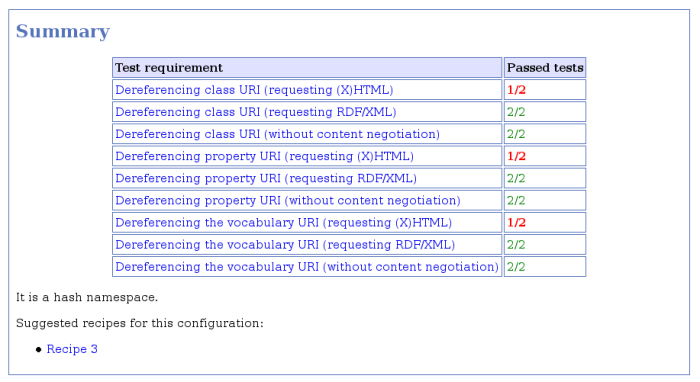
\includegraphics[width=12cm]{images/report-summary.png}
 \caption{\label{fig:report-summary}Example of a report summary made by Vapour.}
\end{figure}

In order to facilitate the testing of the results of content negotiation on a single 
URI, we developed a web-based application called Vapour\footnote{\url{http://vapour.sourceforge.net/}}
that facilitates the task. This service will request the provided vocabulary 
URI from the server and run a test suite specifically designed to test the responses 
of the server against the Recipe specifications. Tests are performed on the covabulary
URI, one class and one property. According to these tests, the system suggests the 
best recipe(s) for your server configuration. It is built upon an in-memory RDF store
that stores all assertions. It uses a combination of EARL~\cite{EARL}, HTTP
Vocabulary~\cite{Koch2007} and an RDF representation of the Recipes. Thus Vapour 
is able to provide reports both in HTML and in RDF. For HTML view the service 
displays a clean and concise pass/fail report on each set of tests 
as  well as a detailed explanation of its  findings (Figure~\ref{fig:report-summary}), 
including a graphical representation of the HTTP dialog used in each test.
For the RDF view %,obviously using content negotiation (FIXMEEEEEEEEEEEEEEEEEE)
the system provide a RDF/XML serialization of the same report.

The project is also available as an online service\footnote{\url{http://idi.fundacionctic.org/vapour}}.

The application has been developed in the Python scripting language, using common
Python libraries such as urllib, httplib, web.py and RDFLib. Scripting languages such 
as Python allow an agile development of applications in short time with little 
resources. The Vapour source code is available on 
SourceForge\footnote{\url{http://sourceforge.net/projects/vapour/}} 
as open source.

\begin{figure}
 \centering
 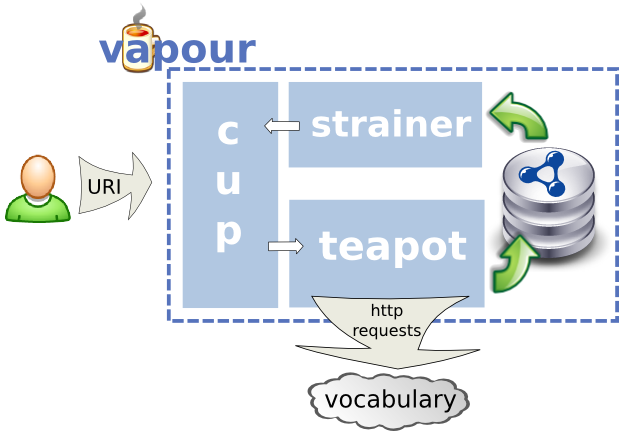
\includegraphics[width=12cm]{images/arch.png}
 \caption{\label{fig:arch}High level architecture of Vapour.}
\end{figure}

As depicted in Figure~\ref{fig:arch}, Vapour has a simple and functional
design that fulfils the objectives of the project. It is composed of three
main components:

\begin{description}

  \item \textbf{cup} is the web front-end. It is built using the web.py framework
        and the Cheetah template engine. It provides a web interface that allows 
        the user to interact with the other components of the platform in a 
        simple way. The system has been designed to allow more types 
        of interfaces and, for instance, we also provide a command line interface.

  \item \textbf{teapot} is the core of the application. It launches
        HTTP dialogs 
        (with and without content negotiation) to evaluate the response
        status code and content-type. It requests the URI of the vocabulary, and 
        also the URIs of a class and a property. All resulting assertions are 
        stored in the RDF store to be serialized later in the interface.

  \item \textbf{strainer} is the module in charge of generating the reports for
        each test performed by teapot. It makes some SPARQL %~\cite{SPARQL} 
        queries on the model to obtain the trace of each test, and it generates 
        a report in XHTML or RDF/XML. For XHTML reports we also use Cheetah 
        templates.

\end{description}

The service can be deployed as a normal CGI behind Apache or using a Python web 
framework. We reviewed the security of the application avoiding some common problems
in this kind of applications, such as limiting requests per client.

\begin{table}
\caption{Ratio of passed tests / total tests for a list of representative vocabularies of the semantic web.}
\centering
\begin{tabular}{lccc}
\hline
Namespace & Accept & Accept & Default \\
 & RDF & HTML & response \\
\hline\hline
\texttt{http://www.w3.org/1999/02/22-rdf-syntax-ns\#} & 3/3 & N/A & RDF/XML \\
\texttt{http://www.w3.org/2000/01/rdf-schema\#} & 3/3 & N/A & RDF/XML \\
\texttt{http://xmlns.com/foaf/0.1/} & 3/3 & 3/3 & HTML \\
\texttt{http://purl.org/dc/elements/1.1/} & 2/2 & 0/2 & RDF/XML \\
\texttt{http://www.w3.org/2003/01/geo/wgs84\_pos\#} & 3/3 & 0/3 & RDF/XML \\
\texttt{http://rdfs.org/sioc/ns\#} & 3/3 & 0/3 & RDF/XML \\
\texttt{http://www.w3.org/2004/02/skos/core\#} & 3/3 & 3/3 & RDF/XML \\
\texttt{http://usefulinc.com/ns/doap\#} & 3/3 & 0/3 & RDF/XML \\
\texttt{http://purl.org/rss/1.0/} & 1/3 & 0/3 & HTML \\
\texttt{http://semantic-mediawiki.org/swivt/1.0\#} & 0/3 & 0/3 & text/plain \\ [1ex]
\hline
\end{tabular}
\label{tab:usage}
\end{table}

\section{\label{sec:experimental}Experimental results}

Practical experimentation illustrates some common problems of how
content negotiation is implemented, and enables the discussion on 
these problems. We checked some RDFS and OWL vocabularies published on the web.
We chose the most frequently used vocabularies, in terms of number of
instances, according to the last scientific study~\cite{Li2005}. However,
this ranking is aging (2004), so we also included some newer
vocabularies, such as SKOS, DOAP and SIOC, which are also popular
according to more up-to-date sources\footnote{See the ranking at http://pingthesemanticweb.com/stats/namespaces.php (retrieved 12/Mar/2008) by PingTheSemanticWeb.com~\cite{Bojars2007}}.

Table~\ref{tab:usage} summarizes the results of running Vapour against a list of
ten representative vocabularies of the semantic web. These results provide an
approximation of the
actual quality of the publication of vocabularies on the web. All the vocabularies
were retrieved on 12/Mar/2008.

For each vocabulary, the vocabulary URI, a class URI and a property URI are tested
(except for Dublin Core, which does not have any class). The results show that
most vocabularies are correctly published as RDF. However, it is significant that
most vocabularies do not correctly serve HTML representations of the resources.
Additionally, some vocabularies return an incorrect MIME type,
such as \texttt{text/plain} or \texttt{application/xml}.

\section{\label{sec:conclusions}Conclusions}

Content negotiation is a dangerous technique. First it appears as some thing very 
simple, but as we have seen it is too easy to make certain mistakes. This is 
further complicated when we have formats embedded within other formats,
such as RDFa~\cite{Birbeck2006}. Scripting languages, and applications such as 
Vapour, are very useful in solving some kind on tasks and provide quality 
assurance in the best possible way.

%FIXME: delete this (off topic) paragraph???
%As we have seen, it is still necessary to solve as soon as possible some 
%important issues in the actual document of the Recipes. While we do not 
%find the most correct way to do it, maybe a \textit{push} action from the Web 
%community will be necessary to develop a new module that allows to serve 
%Linked Data in the correct way with content negotiation.

The application presented in this paper is still a prototype, but  
it already helps to debug how content negotiation is implemented in web servers. One of the 
goals was to provide an RDF serialization of the reports. Using this machine-readable 
format, it should be easy to deploy another service upon it that uses this data for 
other tasks, for example, a service to check the compliance of a specific collection 
of vocabularies published on the Web.


% ---- Bibliography ----
\bibliographystyle{abbrv}
\bibliography{../references}

\end{document}
